\documentclass{article} % For LaTeX2e
\usepackage{nips13submit_e,times}
\usepackage{hyperref}
\usepackage{url}
\usepackage{tikz}
\usepackage{wrapfig}
\usepackage{graphicx}
\usepackage{subcaption}
\usepackage{amsmath}

\usepackage{graphicx}
\usepackage{caption}
%\usepackage{natbib}

\usepackage{array}
\usepackage{booktabs}
\setlength{\heavyrulewidth}{1.5pt}
\setlength{\abovetopsep}{4pt}

\bibliographystyle{natbib}
%\documentstyle[nips13submit_09,times,art10]{article} % For LaTeX 2.09

\title{Learning Human Activities and Object Functionality through Conditional Random Fields}

\author{
Nakul Gopalan\\
Department of Computer Science\\
Brown University\\
Providence, RI 02912 \\
\texttt{ngopalan@cs.brown.edu} \\
\And
Jun Ki~Lee\\
Department of Computer Science\\
Brown University\\
Providence, RI 02912 \\
\texttt{jklee@cs.brown.edu} \\
}

% The \author macro works with any number of authors. There are two commands
% used to separate the names and addresses of multiple authors: \And and \AND.
%
% Using \And between authors leaves it to \LaTeX{} to determine where to break
% the lines. Using \AND forces a linebreak at that point. So, if \LaTeX{}
% puts 3 of 4 authors names on the first line, and the last on the second
% line, try using \AND instead of \And before the third author name.

\newcommand{\fix}{\marginpar{FIX}}
\newcommand{\new}{\marginpar{NEW}}

\nipsfinalcopy % Uncomment for camera-ready version

\begin{document}

\maketitle

\begin{abstract}
Recognizing a human activity is a skill that humans learn early in life. Activity recognition helps humans in predicting next steps of the activity in question and also in planning other activities with respect to the recognized activity. Our goal is to recognize human activities using machine learning, to predict next steps of an action, or provide help using robots or other interfaces. Specifically, what interests us is the human activities being performed near a table-top table or a shelf, where the human can be observed and helped by a robot. We will use a dataset from \cite{koppula2013detectingactivitiesrgbd} to learn a Graphical Model with temporal and spatial structure, which can then be used to predict the action being performed and functionalities of objects. Both can then be used to recognize a higher level activity. First we compare the graph structures used in the original paper to understand the significance of the graph structure used. Further, our efforts in this work are to model the problem as an HMM first and then a CRF (Conditional Random Fields) and compare performance to the original paper in classifying sub-activities. We classify the main activity using a bag of words model with features from the complete activity. 
%We will tackle the problem using Conditional Random Fields and try to achieve better performance.
\end{abstract}

\section{Introduction}
Recognizing a human activity is a skill that humans learn early in life. Activity recognition helps humans in predicting next steps of the activity in question and also in planning other activities with respect to the recognized activity. Our objective is to recognize human activities using machine learning, to predict next steps of an action. Recognized actions can provide help to humans using robots or other interfaces. Specifically of interest to us are the human activities being performed on a table-top, where the human can be observed and helped by a robot.

We use the  dataset\footnote{\url{http://pr.cs.cornell.edu/humanactitivities}} from \cite{koppula2013detectingactivitiesrgbd}
 to learn a Graphical Model with temporal and spatial structure, which can then be used to predict the action being performed and functionalities of objects. The dataset is created from streams of the RGB-D images acquired from a Infrared depth sensing camera. The dataset contains both the tracked human skeletal poses and object locations and supervised labels of sub- and high-level- activities and object functionalities. We first provide some background over the methods used to solve this problem before and an overview of the dataset. Next we alter the original graph structure in \cite{koppula2013detectingactivitiesrgbd} by changing their code and running learning and testing on the new graph structure. Finally we try to predict the sub-activities using linear chain HMMs and CRFs.
 
 
\section{Previous work} 
%Among many works in human activity recognition using RGB-D images, Sung et al. in \citet{sung2012unstructured}
%proposed a hierarchical maximum entropy Markov model to detect high level activities and sub-activities. This work only uses human skeletal data. Gall et al. in \cite{gall2011functional}
% used both the human skeletal data and object tracking data to inference sub-activities and object functionalities. His approach sequentially inferences sub-activities and then object functionalities. It does not take both into account at the same time. Koppula et al. in \cite{koppula2013detectingactivitiesrgbd}
% and \cite{koppula2013anticipating}, uses both the human skeletal poses and object locations and their relationships to low and high level activities and functionalities of objects using Conditional Random Fields (CRF). 

\section{Dataset}
We explored data sets with activity labels and corresponding skeletal trajectories. Humans frequently perform activities using objects, especially in table-top scenarios. The dataset from \cite{koppula2013detectingactivitiesrgbd} was constructed keeping this relationship in mind. The raw data consists of the RGB-D frames from the scenes of humans performing activities and human skeletal poses from the OpenNI NITE tracker \cite{PrimeSense2010}. The dataset has recordings of  $120$ labelled moderate sized human activities of ten types, e.g.: making cereal, microwaving, taking food, etc. The skeletal poses are not precise and have confidence intervals. The labels on the data are related to both the objects present in the scene and the activities involved. Activity specific labels are frame-wise labels on sub-activities and the main activity being performed. The sub-activity labels are that of \textit{reaching, moving, pouring, eating, drinking, opening, placing, closing, scrubbing} and \textit{null}. The object specific data consist of object locations for each time frame per object with its object id and its affordance present in the scene. The object affordance labels are those of \textit{reachable, movable, pourable, pour to, containable, drinkable, openable, placeable, closable, scrubbable} and \textit{stationary}. The dataset also has pre-computed features that have relationship between objects and skeletal poses across frames.  



\begin{figure}
\centering
\hspace{-3mm}
\begin{subfigure}[b]{0.45\textwidth}
\label{fig:model}
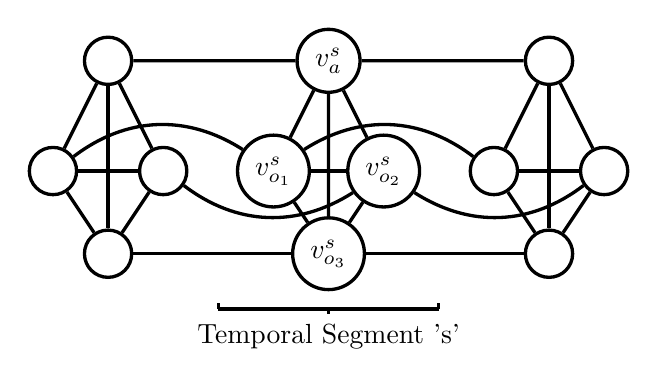
\begin{tikzpicture}[scale=0.7, -,auto,very thick,main node/.style={circle,draw, minimum size=0.6cm}]
  \node[main node] (a1) at (1, 3.5) {};
  \node[main node] (a2) at (1, 0) {};
  \node[main node] (a3) at (0, 1.5) {};
  \node[main node] (a4) at (2, 1.5) {};
  \node[main node] (b1) at (5, 3.5) {$v_a^s$};
  \node[main node] (b2) at (5, 0) {$v_{o_3}^s$};
  \node[main node] (b3) at (4, 1.5) {$v_{o_1}^s$};
  \node[main node] (b4) at (6, 1.5) {$v_{o_2}^s$};
  \node[main node] (c1) at (9, 3.5) {};
  \node[main node] (c2) at (9, 0) {};
  \node[main node] (c3) at (8, 1.5) {};
  \node[main node] (c4) at (10, 1.5) {};
  \path
	(a1) edge (a2)
    (a1) edge (a3)
    (a1) edge (a4)
    (a2) edge (a3)
    (a2) edge (a4)
    (a3) edge (a4)
	(b1) edge (b2)
    (b1) edge (b3)
    (b1) edge (b4)
    (b2) edge (b3)
    (b2) edge (b4)
    (b3) edge (b4)
	(c1) edge (c2)
    (c1) edge (c3)
    (c1) edge (c4)
    (c2) edge (c3)
    (c2) edge (c4)
    (c3) edge (c4)
    (a1) edge (b1)
    (b1) edge (c1)
    (a2) edge (b2)
    (b2) edge (c2)
    (a3) edge [bend left=35] (b3)
    (b3) edge [bend left=35] (c3)
    (a4) edge [bend right=35] (b4)
    (b4) edge [bend right=35] (c4);
  \draw[very thick] (3, -1)--(7, -1);
  \draw[very thick] (3, -1)--(3, -0.9);
  \draw[very thick] (7, -1)--(7, -0.9);
  \draw[very thick] (5, -1)--(5, -1.1);
  \node at (5, -1.5) {Temporal Segment 's'};
\end{tikzpicture}
\end{subfigure}
\hspace{14mm}
\begin{subfigure}[b]{0.45\textwidth}
\label{fig:image}
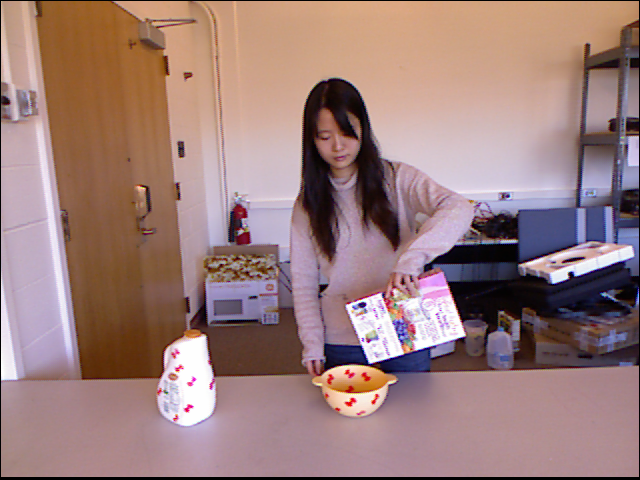
\includegraphics[height=4cm]{images/RGB_137.png}%[height=4cm]
\end{subfigure}
\caption{ \textbf{(a)} an example of a Conditional Random Field used in \cite{koppula2013detectingactivitiesrgbd}. Each temporal segment (s) has one sub-activity node $v_a^s$ and three object nodes $\{ v^s_{o_1}, v^s_{o_2}, v^s_{o_3} \}$, \textbf{(b)} an example image from the data set}
\end{figure}


\section{Methods}
The data from \cite{koppula2013detectingactivitiesrgbd} has both temporal and spatial structure. For example, the spatial structure has relationships between objects and skeleton positions within a frame. There is also a temporal relationship between previous skeletal pose and object positions and those of the current frame. The authors from \cite{koppula2013detectingactivitiesrgbd} modeled this structure using a pairwise Conditional Random Field(\cite{sutton06introduction}) as shown in 
Fig.~\ref{fig:model}. 
Here each node corresponds to an object or a sub-activity. The object nodes can take any of the $12$ possible affordance labels and the sub-activity nodes can take any of the $10$ possible labels. The affordance and subactivity nodes are hidden, but feature values for label assignments over the nodes can be computed. The authors in \cite{koppula2013detectingactivitiesrgbd} first segmented an input activity, or set of frames into segments that are more likely to belong to a single sub-activity. The authors used a sum of Euclidean distance between joints metric to judge the change in sub-activities. The threshold to split sub-activities seems to be based on a trial and error heuristic. The sub-activities are temporally linked giving a chain graph structure as shown in Fig.~\ref{fig:model}. The authors used this graph structure to predict sub-activity labels and object affordances by performing inference over the model, and then used an SVM to predict the label of the over all activity. To predict the sub-activity and object affordance labels the authors used a maximum energy formulation, where the labels that lead to the maximum possible energy together are accepted. This energy is a sum of products of features and feature weights. The energy function requires learning the weights of the features first, with the supervised labeled input from the dataset discussed above, such that training error is minimized. 


\section{Importance of graph structures}
The original paper by \cite{koppula2013detectingactivitiesrgbd} uses the graph structure shown in Fig.~\ref{fig:model}. The sub-activity nodes and object affordance nodes are completely connected within a temporal segment. The authors infer the series of sub-activities as an argmax over an energy function for the linear chain that describes the sequence of sub-activities:


\begin{figure}
        \centering
        \begin{subfigure}[b]{0.45\textwidth}
                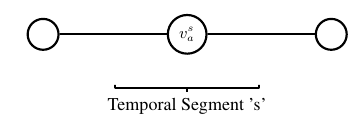
\includegraphics[width=\textwidth]{model_simple}
                \caption{Graph with only sub-activity labels}
                \label{fig:model_simple}
        \end{subfigure}%
        ~ %add desired spacing between images, e. g. ~, \quad, \qquad, \hfill etc.
          %(or a blank line to force the subfigure onto a new line)
        \begin{subfigure}[b]{0.45\textwidth}
                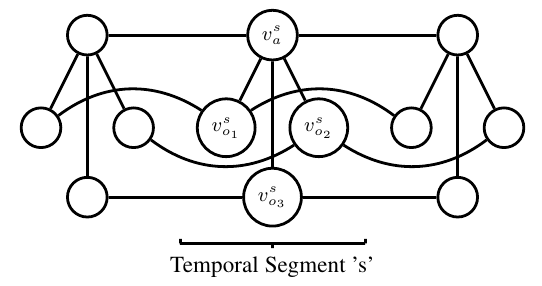
\includegraphics[width=\textwidth]{model_no_oo}
                \caption{Graph with no object - object edges}
                \label{fig:model_no_oo}
        \end{subfigure}
       
        \caption{Different graph structures tried}
        \label{fig:graph_structures}
\end{figure}

\begin{gather}
\hat{\mathbf{y}} = \arg\!\max_{\mathbf{y}} E_{\mathbf{w}} (\mathbf{x},
\mathbf{y})\\
E_{\mathbf{w}} (\mathbf{x}, \mathbf{y}) = E_o + E_a + E_{oo} + E_{oa}
+ E^t_{oo} + E^t_{oa} \\
E_o = \sum\limits_{i \in \mathcal{V}_o} \psi_o(i) = \sum\limits_{i \in
\mathcal{V}_o} \sum\limits_{k \in K_o}y^k_i \left[
\mathbf{w}^k_{\mathbf{o}} \cdot \phi_o(i) \right] \\
E_a = \sum\limits_{i \in \mathcal{V}_a} \psi_a(i) = \sum\limits_{i \in
\mathcal{V}_a} \sum\limits_{k \in K_a}y^k_i \left[
\mathbf{w}^k_{\mathbf{a}} \cdot \phi_a(i) \right] \\
E_{oo} = \sum\limits_{(i,j) \in \mathcal{E}_{oo}} \sum\limits_{(l,k)
\in K_o \times K_o} y^l_i y^k_j \left[ \mathbf{w}^{lk}_{\mathbf{oo}}
\cdot \phi_{oo}(i,j) \right] \\
E_{oa} = \sum\limits_{(i,j) \in \mathcal{E}_{oa}} \sum\limits_{(l,k)
\in K_o \times K_a} y^l_i y^k_j \left[ \mathbf{w}^{lk}_{\mathbf{oa}}
\cdot \phi_{oa}(i,j) \right] \\
E^t_{oo} = \sum\limits_{(i,j) \in \mathcal{E}^t_{oo}}
\sum\limits_{(l,k) \in K_o \times K_o} y^l_i y^k_j \left[
\mathbf{w}^{t^{lk}}_{\mathbf{oo}} \cdot \phi^t_{oo}(i,j) \right] \\
E^t_{aa} = \sum\limits_{(i,j) \in \mathcal{E}^t_{aa}}
\sum\limits_{(l,k) \in K_a \times K_a} y^l_i y^k_j \left[
\mathbf{w}^{t^{lk}}_{\mathbf{aa}} \cdot \phi^t_{aa}(i,j) \right]
\end{gather}

where $E_w(\mathbf{x},\mathbf{y})$ is the total energy over all the temporal segments in the activity, $\mathbf{x}$ are the features and $\mathbf{y}$ are the sub-activity and object affordance labels. $\hat{\mathbf{y}}$ is the inferred series of object affordance and sub-activity labels. $V_a$ and $V_o$ are the sub-activity and object nodes of the graph. $K_a$ and $K_o$ are the sub-activity and object affordance labels that the nodes can take. $E_o$ and $E_a$ are the energy functions over individual nodes, i.e., sums over all the nodes taking on all possible combinations of the labels $y^k$ with given features $\phi$, when the weights of the nodes for label $k$ are $\mathbf{w}^k$. Further there are energy terms over the edges of the graph $E_{oo}$ and $E_{oa}$ that sum over all possible combination of labels between object - object nodes or object - sub-activity nodes at each temporal segment, given features and weights. These represent the relationship between object affordances and object affordance and sub-activities.  There are also temporal energy terms of $E_{oo}^{t}$ and $E_{aa}^{t}$ that represent the temporal relationship between different sub-activity labels or different object affordance labels, w.r.t. the labels and features of the temporal segment. 

During learning the weights $\mathbf{w}$ are learned such that the error between the predicted label $\hat{\mathbf{y}}$ and true label $\mathbf{y}$  is minimized. Koppula et al. \cite{koppula2013detectingactivitiesrgbd} formulate this problem like a Structural Support Vector Machine problem, which is a convex quadratic problem, and solve it using the cutting plane algorithm. Further after learning the weights, inference is performed using the learned weights to predict the most likely sequence of sub-activities. This inference is performed using mixed integer programming.


We tried to understand the importance of the edges in the graph structure in predicting sub-activity labels. First we performed learning on the original graph Fig.~\ref{fig:model} with the author's source code. The sub-activity labels were predicted correctly $89\%$ of the times as shown in the Table~\ref{table:graphComparison}. Next we removed all dependence of the graph on the object affordance labels,  by tying the weights related to the object affordance nodes to zero, and not performing learning over these weights. We get a linear chain graph in this case, Fig~\ref{fig:model_simple}, and the precision results were $76\%$ clearly lower than those with the object-affordance labels. Further we added back edge weights between sub-activities and object nodes but not between object - object nodes: Fig~\ref{fig:model_no_oo}. We noticed that this lead to a large increase in the precision number to $88\%$. Hence the object-object edges within the same temporal segment in the graph are useful for about $1\%$ increase in precision. 

In this section we looked at the importance of graph structure in solving this inference problem. Next we look at the importance of temporal segmentation in learning and inference.




% For this first during the learning phase we tied the weights realted to the object affordance nodes to zero, and did not perform learning on them. T




\begin{table}[tbp]
\centering
\caption{Comparison of Results with different graph structures.}
\label{table:graphComparison}
\begin{tabular}{*5c}
\toprule
Graph structure &  \multicolumn{2}{c}{Object Affordances} & \multicolumn{2}{c}{Sub-activity Labels}\\
\midrule
{}   & Precision   & Recall    & Precision   & Recall\\
Sub-activity Only   &  NA & NA   & 76\%  & 76\%  \\
Sub Activity and Object Affordances (No Obj-Obj Relationships)   &  87\%   & 87\%     & 88\%    & 88\%  \\
Full Model   &  92\%    &  92\%     & 89\%    & 89\%  \\
\bottomrule
\end{tabular}
\end{table}




\section{Modeling without temporal segments using a simple HMM}
The idea for this experiment was that the simplest way to formulate this problem would be an HMM over all the frames of the data, and predicting the hidden state, i.e., the sub-activity label per frame instead of predicting them for a temporal segment. We performed a training-test split of $2:1$ and learned transition probability between states and observation probabilities of skeletal features. Since the skeletal features were sparse we reduced them to low $10$ dimensional features using clustering. What we noticed immediately was that the transition matrix was almost an identity matrix as there are very few transitions between frames from one sub-activity to another, and far higher self transitions. This lead to the output predictions of sub-activity for all frames being stuck to the most likely sub-activity, producing a low result of $16\%$ accuracy where $10\%$ is chance. We next try to train a CRF based model for temporally segmented data.


%add Jun's things here!





\section{Na{\"i}ve Activity Detection}
\begin{figure}[tpb]
  \centering
    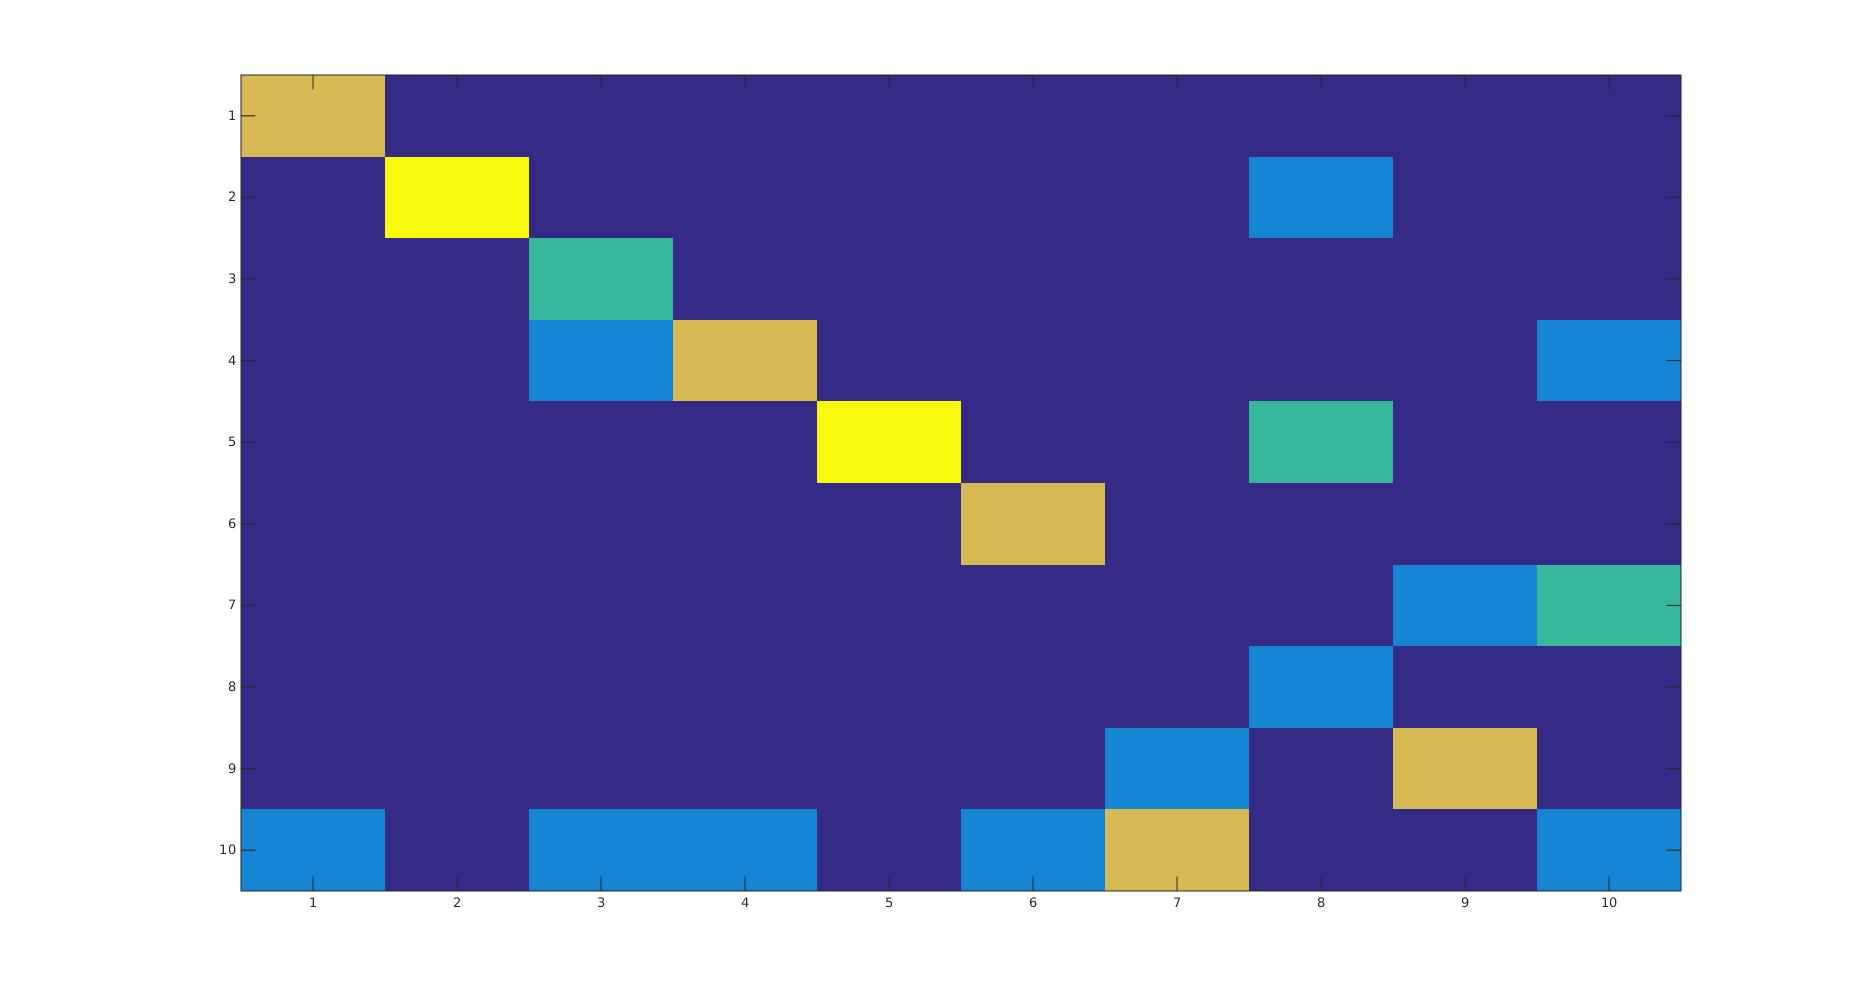
\includegraphics[width=0.8\textwidth]{images/confMat}
    \caption{Confusion Matrix of the high level activity classification using Bag of Words model. The label order is - arranging objects, cleaning, having meal, making cereal, microwaving food, picking objects, stacking, taking food, taking medicine, unstacking objects}
    \label{fig:confmat}
\end{figure}
We classify high level activities from skeletal trajectories using a Bag of Words model \cite{Sivic03} with skeletal poses as features. For each type of activity we have about $12$ examples in the dataset. We use about $8$ examples per activity for training and $4$ examples per activity for testing. Each frame has a skeletal pose, of about $170$ dimensions, and each activity has about $400$ frames. We cluster skeletal poses over all training activities into $200$ clusters using k-means. Further for each activity label we create a histogram by counting number of skeleton frames of an activity in each of the $200$ clusters.  Next for each test activity we find the nearest neighbor word from the trained histogram words and return its label. The accuracy of this simple Bag of Words model is about $67.3\%$.  The original paper cites an accuracy of $75\%$ in recognizing these high level activities, but when we ran experiments with their current code base this number was higher than $90\%$. The confusion matrix for this classification is show in Fig~\ref{fig:confmat}. It can clearly been seen that there is confusion in classification of the activity labels of stacking and unstacking as differentiating between these labels needs temporal information. Similar confusion was also seen in the original paper.

\section{Conclusion}
In this work we tried different methods to learn the hidden labels of sub-activities given the dataset from \cite{koppula2013detectingactivitiesrgbd}. We saw that changing the graph structure w.r.t. to the original formulation leads to a drop in performance. The temporal segmentation of frames is a key requirement in this framework. Further that na{\"i}ve methods like bag of words models can go a long way in guessing high level activity labels.



\bibliography{ref}

\end{document}
